\documentclass[11pt]{article}

\usepackage[margin=2cm]{geometry}

\usepackage{graphicx}

\usepackage{booktabs}

\usepackage{longtable}

\usepackage{hyperref}

\usepackage[T1]{fontenc}

\usepackage[utf8]{inputenc}

\title{Universo foco textil produccion y lavado 2026}

\author{Proyecto Atoyac - salida reproducible}

\date{\today}

\begin{document}

\maketitle

\section{Proposito}

Este reporte documenta un universo operativo amplio llamado \texttt{foco\_textil\_produccion\_y\_lavado\_2026}. El objetivo es integrar, desde DENUE 2026, establecimientos con senales de produccion textil, maquila, confeccion, mezclilla, lavado, tintoreria, acabado o tratamiento. No es evidencia de descarga, contaminacion ni incumplimiento; es una herramienta de priorizacion y auditoria.

\section{Criterio de construccion}

La base fue \texttt{data/processed/denue2026\_universo\_textil\_clasificado.gpkg}. Se excluyeron decisiones automaticas de comercio, renta y no pertinencia. Se incluyeron registros con senales de proceso humedo/lavado/acabado, mezclilla, maquila/confeccion, fabricacion textil o pendientes de revision textil. Dentro del universo se conserva una categoria interna para distinguir lavado/acabado de maquila/confeccion.

\section{Resultados}

El universo foco contiene 356 registros.

\subsection{Conteo por categoria}

\begin{tabular}{ll}
\toprule
categoria\_foco\_textil & registros \\
\midrule
lavado\_acabado\_proceso\_humedo & 38 \\
maquila\_confeccion\_textil & 278 \\
mezclilla\_produccion & 38 \\
textil\_pendiente\_revision & 2 \\
\bottomrule
\end{tabular}

\subsection{Conteo por localidad}

\begin{tabular}{ll}
\toprule
localidad & registros \\
\midrule
Santa Ana Xalmimilulco & 340 \\
Rancho de los Caballos & 10 \\
Los Volcanes & 2 \\
La Concepcin & 1 \\
El Carmen [Parque Industrial] & 1 \\
Centro Logstico [Reserva Industrial] & 1 \\
Los Encinos & 1 \\
\bottomrule
\end{tabular}

\subsection{Membresias con otros universos}

\begin{tabular}{ll}
\toprule
conjunto & registros \\
\midrule
foco\_textil\_produccion\_y\_lavado\_2026 & 356 \\
en\_universo\_prioritario\_2026 & 52 \\
en\_universo\_prioritario\_actual & 46 \\
en\_mh\_filtrado & 42 \\
\bottomrule
\end{tabular}

\subsection{Comparacion con MH filtrado}

\begin{tabular}{ll}
\toprule
comparacion\_mh\_foco & registros \\
\midrule
foco\_y\_mh & 42 \\
mh\_sin\_id & 6 \\
solo\_foco & 314 \\
solo\_mh & 1 \\
\bottomrule
\end{tabular}

\section{Mapas}

\begin{figure}[h!]\centering

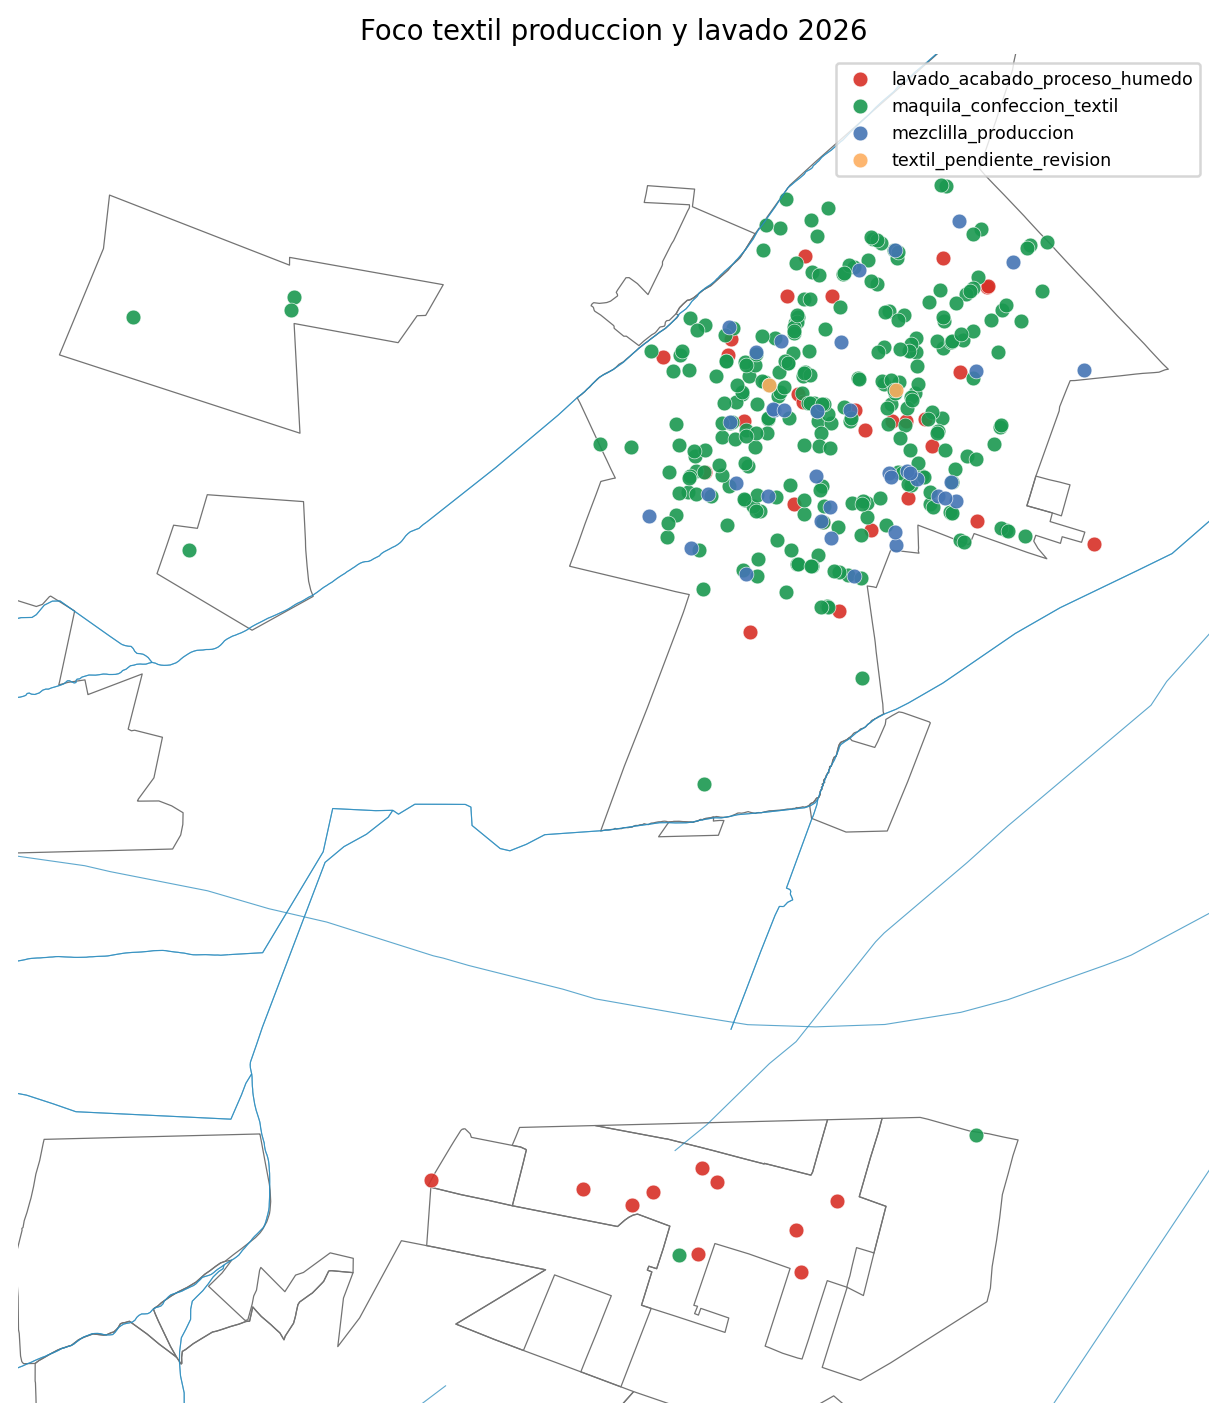
\includegraphics[width=0.95\linewidth]{../mapas/mapa_foco_textil_por_categoria.png}

\caption{Universo foco textil produccion y lavado 2026 por categoria interna.}

\end{figure}

\begin{figure}[h!]\centering

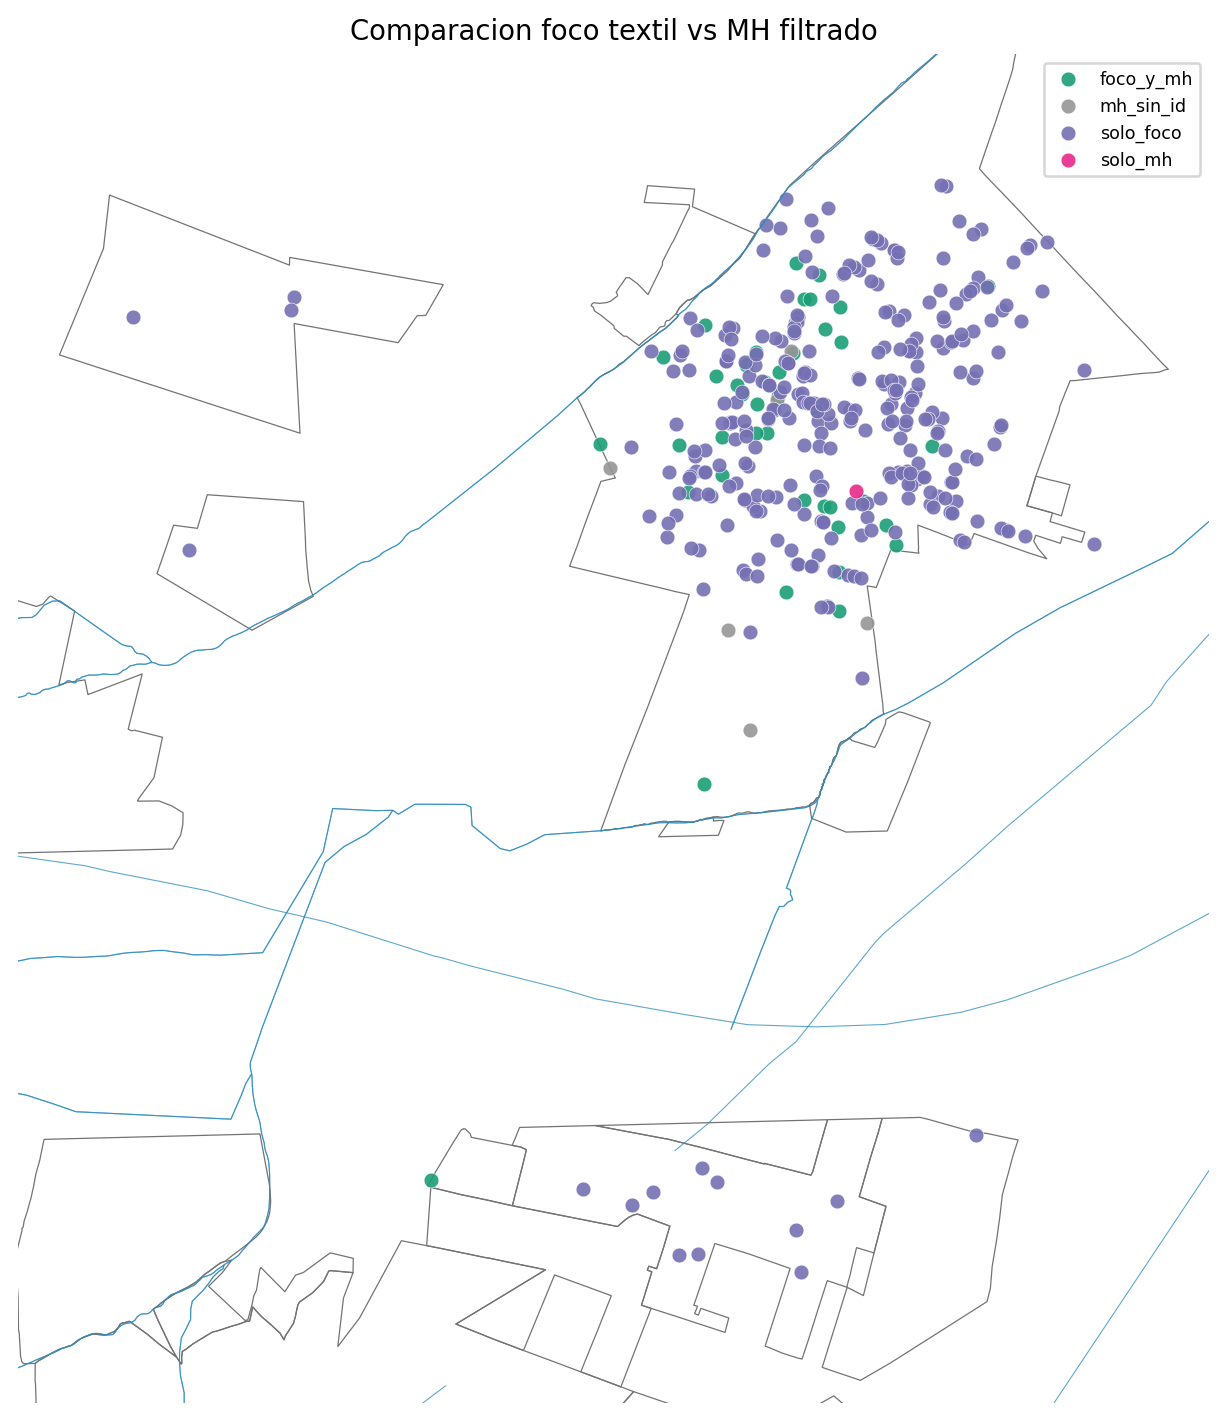
\includegraphics[width=0.95\linewidth]{../mapas/mapa_comparacion_foco_vs_mh.png}

\caption{Comparacion entre universo foco y capa MH filtrada.}

\end{figure}

\section{Lectura comparativa}

La capa MH filtrada se solapa parcialmente con este universo, pero tambien contiene registros fuera del foco y algunos puntos sin ID DENUE. Esto sugiere que MH captura una nocion mas amplia de talleres o maquilas textiles. El nuevo universo foco permite dialogar con ese criterio amplio sin abandonar la trazabilidad por senales: produccion/confeccion, mezclilla y lavado/acabado quedan separados en campos auditables.

\section{Archivos generados}

\begin{itemize}

\item \texttt{capas\_qgis/foco\_textil\_produccion\_y\_lavado\_2026.gpkg}

\item \texttt{tablas/foco\_textil\_produccion\_y\_lavado\_2026.csv}

\item \texttt{tablas/comparacion\_foco\_vs\_mh.csv}

\item \texttt{mapas/mapa\_foco\_textil\_por\_categoria.html}

\item \texttt{mapas/mapa\_comparacion\_foco\_vs\_mh.html}

\end{itemize}

\section{Conclusion}

El universo prioritario previo sigue siendo mas estricto para estudio ambiental. El universo foco textil produccion y lavado es un producto complementario, mas amplio, util para revisar talleres, maquilas y establecimientos con posible relacion productiva textil. Debe usarse como capa de trabajo y auditoria, no como prueba de contaminacion.

\end{document}